% ============================================================
% GELLS-DEM: Cell-Driven Granular Scaffold Remodeling
% PNAS-format manuscript
% ============================================================
\documentclass[9pt,twocolumn,twoside]{pnas-new}

% --- Packages ---
\usepackage{amsmath}
\usepackage{graphicx}
\usepackage{microtype}
\usepackage{booktabs}
\usepackage{siunitx}
\usepackage{xcolor}
\usepackage{natbib}
\usepackage{hyperref}

\graphicspath{{figures/}}

% --- Convenience macros ---
\newcommand{\phif}{\phi_\mathrm{f}}
\newcommand{\phii}{\phi_\mathrm{i}}
\newcommand{\phiv}{\phi_\mathrm{v}}
\newcommand{\phiRCP}{\phi_\mathrm{RCP}}
\newcommand{\phiJ}{\phi_\mathrm{J}}
\newcommand{\xf}{x_\mathrm{f}}
\newcommand{\xistar}{\xi^{*}}
\newcommand{\Gtilde}{\tilde{G}}
\newcommand{\sigmacell}{\sigma_\mathrm{cell}}
\newcommand{\sigmazero}{\sigma_0}
\newcommand{\sigmay}{\sigma_\mathrm{y}}
\newcommand{\etaeff}{\eta_\mathrm{eff}}
\newcommand{\um}{\,\si{\micro\metre}}
\newcommand{\nN}{\,\si{nN}}
\newcommand{\kPa}{\,\si{kPa}}

% ============================================================
% Front matter
% ============================================================

\title{Cell-Driven Remodeling of Granular Hydrogel Scaffolds:\\
A Discrete Element Model with Free Energy Landscape Analysis}

\author{Alexander D.\ McGhee\textsuperscript{a,1}}

\affil[a]{Department of Mechanical Science and Engineering, University of Illinois at Urbana-Champaign, Urbana, IL 61801}

\leadauthor{McGhee}
\correspondingauthor{\textsuperscript{1}To whom correspondence should be addressed. E-mail: amcghee2@illinois.edu}

\significancestatement{
Granular hydrogel scaffolds---jammed packings of soft microparticles---are a
promising platform for engineering tissues with controlled microarchitecture.
When cell-laden (functional) granules are mixed with passive (inert) granules,
cells generate traction forces that compact the functional phase, producing
programmable shape transformations. We present a discrete element method (DEM)
simulation that captures the essential physics of this process---Hertzian
contact, motor-clutch cell traction, area-dependent friction, and
superellipsoidal granule shapes---together with a mean-field compaction model
and a free energy landscape framework that decomposes the competition between
cell driving and mechanical resistance into six physical mechanisms. The
resulting design rules map scaffold parameters to tissue architectures
spanning bone, mucosa, kidney, and cardiac muscle.}

\authorcontributions{A.D.M.\ designed the study, developed the simulation
code, performed the analysis, and wrote the paper.}

\keywords{granular hydrogels $|$ discrete element method $|$ tissue
engineering $|$ energy landscape $|$ cell mechanics}

\pnasabstract{Granular hydrogel scaffolds composed of jammed hydrogel microparticles
provide a versatile platform for tissue engineering, offering tunable
porosity, mechanics, and biological function. When a fraction of the granules
are laden with cells (functional) and the remainder are passive (inert),
cell-generated traction forces drive selective compaction of the functional
phase, producing macroscopic shape transformations. Here we develop
GELLS-DEM, a two- and three-dimensional overdamped discrete element method
that resolves individual granule contacts through Hertzian mechanics,
motor-clutch cell traction, area-dependent hydrogel friction, DMT adhesion,
and superellipsoidal particle shapes. We derive a volume-conserving two-zone
mean-field model that reduces the many-body DEM dynamics to a single
ordinary differential equation for the compaction coordinate $\xi$, and
construct a free energy landscape $\tilde{G}(\xi)$ decomposed into six
competing physical mechanisms: cell traction, Hertzian elastic resistance,
Herschel-Bulkley yield stress near jamming, osmotic void redistribution,
inert-granule geometric frustration, and functional--inert interfacial
tension. Five dimensionless groups---the cell--elastic ratio $\beta$,
cellular capillary number Ca, inert fraction $\Phi_r$, packing
proximity $\Psi$, and interfacial number $\Gamma$---govern the landscape
topology and determine the equilibrium compaction $\xi^{*}$. A 5000-sample
Latin hypercube parameter sweep maps the scaffold design space to tissue
architectural descriptors, yielding quantitative design rules for achieving
target organ microstructures including trabecular bone ($\xi^{*} \approx 0.58$),
intestinal mucosa ($\xi^{*} \approx 0.38$), kidney cortex
($\xi^{*} \approx 0.21$), and cardiac muscle ($\xi^{*} \approx 0.10$).}

\dates{This manuscript was compiled on \today.}

\begin{document}

\maketitle
\thispagestyle{firststyle}

% ============================================================
\section*{Introduction}
% ============================================================

Granular hydrogels---dense packings of soft polymeric microparticles---have
emerged as a versatile class of biomaterials for tissue repair and
regeneration \cite{Riley2019}. Unlike monolithic hydrogels, granular
scaffolds possess inherent porosity at the inter-particle scale, enabling
nutrient transport, cell migration, and waste removal without the need for
engineered pore networks \cite{Hollister2005}. The mechanical properties of
these scaffolds are governed by the Hertzian contacts between individual
building blocks rather than by the bulk polymer network, providing an
additional axis of tunability through particle stiffness, size, and shape
\cite{Cai2022}.

A particularly compelling application is the use of biphasic granular
composites in which cell-laden ``functional'' granules are mixed with passive
``inert'' granules at a prescribed ratio \cite{DiCaprio2025}. Cells within
the functional phase generate traction forces through the motor-clutch
mechanism \cite{Chan2008,Bangasser2013}, forming intercellular bridges that
compact the functional granules while the inert phase resists rearrangement.
The resulting differential compaction produces macroscopic shape
transformations whose geometry depends on the spatial distribution and volume
fraction of each phase.

Despite the promise of this approach, rational design of granular scaffolds
for specific tissue architectures remains largely empirical. The challenge is
fundamentally multi-physics: cell-generated forces must overcome elastic
resistance from Hertzian contacts, yield stress from the jammed packing
\cite{OHern2003,vanHecke2010}, friction between granule surfaces
\cite{Gong2006,Pitenis2014}, and geometric constraints from the inert phase.
A predictive framework requires both a particle-resolved simulation that
captures these interactions and a reduced-order model that identifies the
governing dimensionless groups.

Here we present GELLS-DEM (Granular Encapsulated Living-cell Laden
Scaffold---Discrete Element Method), a simulation framework that addresses
both needs. The DEM engine resolves the overdamped dynamics of $N \sim
500$--$1000$ superellipsoidal granules with Hertzian contact mechanics,
motor-clutch cell traction, area-dependent friction, and DMT adhesion. A
mean-field compaction model reduces the many-body dynamics to a single ODE
for the functional zone fraction $\xf$. Finally, a free energy landscape
analysis decomposes the total free energy into six competing mechanisms,
yielding five dimensionless groups that govern scaffold behavior.

% ============================================================
\section*{Model Formulation}
% ============================================================

\subsection*{Discrete Element Method.}

We model the granular scaffold as a collection of $N$ particles in an
overdamped regime appropriate for microscale dynamics in viscous media
($\mathrm{Re} \ll 1$) \cite{Purcell1977}. Each granule $i$ has position
$\mathbf{x}_i$, radius $R_i$ (or semi-axes $a_i, b_i, c_i$ and blockiness
exponents $n_{1,i}, n_{2,i}$ for superellipsoids), and type $g_i \in
\{0, 1\}$ distinguishing functional ($g_i = 0$) from inert ($g_i = 1$).
The equation of motion is
%
\begin{equation}\label{eq:eom}
  \gamma_i \frac{d\mathbf{x}_i}{dt} = \sum_j \mathbf{F}_{ij}^\mathrm{contact}
  + \mathbf{F}_i^\mathrm{cell} + \mathbf{F}_i^\mathrm{wall},
\end{equation}
%
where $\gamma_i = \gamma_0 R_i$ is the drag coefficient scaled by particle
size. The contact force between particles $i$ and $j$ comprises three
components: Hertzian repulsion, DMT adhesion, and area-dependent tangential
friction. Integration is by forward Euler with a velocity cap to prevent
numerical blowup.

\textit{Hertzian contact.}
For two elastic spheres with overlap $\delta_{ij} = R_i + R_j -
|\mathbf{x}_i - \mathbf{x}_j|$, the normal repulsive force follows Hertz
theory \cite{Johnson1985}:
%
\begin{equation}\label{eq:hertz}
  F_\mathrm{Hertz} = \tfrac{4}{3} E^{*} \sqrt{R^{*}}\, \delta^{3/2},
\end{equation}
%
where $E^{*} = E/[2(1 - \nu^2)]$ is the effective modulus and $R^{*} = R_i
R_j/(R_i + R_j)$ is the reduced radius. For superellipsoidal particles, the
common-normal method \cite{Delaney2010,Jaklic2000} determines the contact
point, penetration depth, and local curvature radii $R_{\mathrm{loc},i}$,
$R_{\mathrm{loc},j}$, which replace the global radii in Eq.~\ref{eq:hertz}.
A Newton-Raphson solver (typically 4--8 iterations) finds the contact
parameters, with a fast-path bypass for sphere--sphere contacts.

\textit{DMT adhesion.}
Normal attractive forces follow the Derjaguin-Muller-Toporov model
\cite{Derjaguin1975}, $F_\mathrm{adh} = 2\pi W R^{*}$, where the work of
adhesion $W$ depends on surface chemistry: bare--bare ($W = 0.5$\,mJ/m$^2$),
bare--collagen ($W = 1.0$\,mJ/m$^2$), and collagen--collagen ($W =
2.0$\,mJ/m$^2$). These values are deliberately conservative to maintain
the small-overlap assumption ($\delta/R < 0.1$).

\textit{Area-dependent friction.}
Hydrogel-on-hydrogel friction is fundamentally area-dependent rather than
load-dependent \cite{Gong2006,Pitenis2014,Uruena2018}: $F_\mathrm{fric} =
\tau_0 A_\mathrm{contact} \tanh(v_t / v_\mathrm{ref})$, where the
interfacial shear stress $\tau_0$ ranges from $50$\,Pa (bare gemini) to
$2000$\,Pa (collagen--collagen) and $A_\mathrm{contact} = \pi R^{*} \delta$
is the Hertzian contact area.

\textit{Motor-clutch cell traction.}
Cells on functional granules generate traction through the motor-clutch
mechanism \cite{Chan2008,Bangasser2013}. Each cell exerts a force
%
\begin{equation}\label{eq:mc}
  F_\mathrm{mc} = F_\mathrm{stall} \cdot
  \frac{k_\mathrm{sub}}{k_\mathrm{sub} + k_\mathrm{opt}} \cdot
  \alpha_\mathrm{FA} \cdot f_\mathrm{engage},
\end{equation}
%
where $F_\mathrm{stall} = n_\mathrm{motors} \times F_\mathrm{motor}$ is the
total stall force, $k_\mathrm{sub} = \pi E a_\mathrm{cell} / (1 - \nu^2)$
is the substrate spring constant at the cell scale, $k_\mathrm{opt} =
n_\mathrm{clutches} \times k_\mathrm{clutch}$ is the optimal clutch stiffness,
$\alpha_\mathrm{FA} \in [0,1]$ is focal adhesion maturity
\cite{Geiger2009}, and $f_\mathrm{engage} = k_\mathrm{on}/(k_\mathrm{on} +
k_\mathrm{off})$ is the steady-state clutch engagement fraction. The net
cell force on each granule is the vector sum of all attached cells directed
toward the nearest functional neighbor.

\textit{Cell lifecycle.}
Cells are tracked individually through five states: ATTACHED $\to$ SPREADING
$\to$ PROLIFERATING $\to$ BRIDGING $\to$ SENESCENT \cite{Engler2006}. Cells
attach to collagen-coated functional granule surfaces, spread from
$20\um$-diameter spheres to $5\um$-tall ellipsoids (volume-conserving), and
form intercellular bridges between neighboring functional granules via a
Poisson process with rate $k_\mathrm{bridge}$. Bridges ramp force over a
formation time, persist across timesteps, and transition to senescence after
sustained load.

\textit{Superellipsoidal shapes.}
Granule shape is parameterized as superellipsoids
$\left(|x/a|^{n_1} + |y/b|^{n_1}\right)^{n_2/n_1} + |z/c|^{n_2} = 1$
\cite{Liu2025,Yuan2019}, where semi-axes $(a, b, c)$ control size and aspect
ratio while blockiness exponents $(n_1, n_2)$ interpolate between ellipsoids
($n = 2$) and rounded cuboids ($n > 2$). Rotational dynamics follow
overdamped quaternion integration, with torques arising from off-center
contact forces.

% ============================================================
\subsection*{Mean-Field Compaction Model.}

The $N$-body DEM dynamics can be coarse-grained to a single scalar: the
functional zone fraction $\xf(t) = V_\mathrm{f}/(V_\mathrm{f} +
V_\mathrm{i})$, where $V_\mathrm{f}$ and $V_\mathrm{i}$ are the volumes
occupied by the functional and inert zones, respectively. We define the
compaction coordinate $\xi = 1 - \xf / x_{\mathrm{f},0} \in [0, \xi_\mathrm{max}]$,
where $x_{\mathrm{f},0}$ is the initial zone fraction and
$\xi_\mathrm{max}$ is set by the close-packing limit.

The total solid fraction $\phi_\mathrm{solid} = \phif + \phii$ is
conserved. As the functional zone compacts ($\xi$ increases), its local solid
fraction rises while void fraction decreases; simultaneously, the inert zone
dilates to accommodate the displaced void space. The volume-conserving
constraint yields the local void fractions:
%
\begin{equation}\label{eq:void}
  \phi_{\mathrm{v},\mathrm{f}} = 1 - \frac{\phi_\mathrm{f,0}}{x_{\mathrm{f},0}(1 - \xi)}, \qquad
  \phi_{\mathrm{v},\mathrm{i}} = 1 - \frac{\phi_\mathrm{i,0}}{1 - x_{\mathrm{f},0}(1 - \xi)}.
\end{equation}

The overdamped dynamics of $\xi$ follow from a balance of the cell driving
stress and mechanical resistance \cite{Kramers1940,Doi1986}:
%
\begin{equation}\label{eq:mf_ode}
  \etaeff \frac{d\xi}{dt} = \underbrace{\sigmacell(t)}_{\text{cell driving}}
  - \underbrace{\sigmazero \max(0, \xi - \xi_\mathrm{c})^\alpha}_{\text{elastic resistance}},
\end{equation}
%
where $\sigmacell(t) = \sigma_\infty \cdot f_\mathrm{bridge}(t) \cdot
m(t)$ incorporates the time-dependent bridge formation fraction and focal
adhesion maturity, $\sigmazero = 0.005 E^{*}$ is the elastic resistance
prefactor (calibrated to the DEM Hertzian response), and
$\xi_\mathrm{c}$ is the onset compaction above which elastic contacts form.
The effective viscosity $\etaeff$ and exponent $\alpha$ are fitted to
DEM simulations.

% ============================================================
\subsection*{Free Energy Landscape.}

To understand \textit{why} a given set of scaffold parameters produces a
particular compaction, we construct a free energy $G(\xi)$ whose minimum
$\xistar$ gives the equilibrium compaction \cite{Wales2003}. The landscape
is decomposed into six physically distinct contributions:

\textit{(i) Cell traction} (driving):
\begin{equation}\label{eq:Gcell}
  G_\mathrm{cell}(\xi) = \sigmacell \ln(1 - \xi),
\end{equation}
the only term that decreases monotonically with $\xi$, providing the
thermodynamic driving force for compaction. The logarithmic form arises from
the volume-conserving geometry: $d\xf/d\xi = -x_{\mathrm{f},0}$, so the
work done per unit compaction diverges as $\xi \to 1$.

\textit{(ii) Hertzian elastic resistance}:
\begin{equation}\label{eq:Gelastic}
  G_\mathrm{elastic}(\xi) = \frac{\sigmazero}{2}\,\max(0, \xi - \xi_\mathrm{c})^2,
\end{equation}
obtained by integrating the elastic resistance stress from
Eq.~\ref{eq:mf_ode}. The parabolic form is consistent with Hertzian scaling
in the small-overlap regime.

\textit{(iii) Herschel-Bulkley yield stress}:
\begin{equation}\label{eq:Gyield}
  G_\mathrm{yield}(\xi) = c_\mathrm{y}\, \sigmazero\, \max(0, \xi - \xi_\mathrm{J})^\Delta,
\end{equation}
where $\xi_\mathrm{J}$ is the compaction coordinate corresponding to the
jamming transition ($\phi_\mathrm{f,local} = \phiJ$), $\Delta = 3/2$ is
the O'Hern scaling exponent for Hertzian particles \cite{OHern2003}, and
$c_\mathrm{y} = 0.25$ \cite{Olsson2007,Olsson2012}.

\textit{(iv) Osmotic void redistribution}:
\begin{equation}\label{eq:Gvoid}
  G_\mathrm{void}(\xi) = \Pi \bigl[\Delta\phi_{\mathrm{v,f}}^2\, \xf
  + \Delta\phi_{\mathrm{v,i}}^2\, x_\mathrm{i}\bigr],
\end{equation}
where $\Pi = 3\sigmacell$ is the osmotic pressure scale and
$\Delta\phi_\mathrm{v}$ measures the deviation of local void fraction from
its initial value in each zone \cite{Biot1941,Princen1986}. This term
penalizes the asymmetric redistribution of void space during compaction.

\textit{(v) Inert geometric frustration}:
\begin{equation}\label{eq:Ginert}
  G_\mathrm{inert}(\xi) = k_\mathrm{f}\,
  \frac{\phii}{\phif}\,\xi^2,
\end{equation}
where $k_\mathrm{f} = 1.5\sigmacell$ captures the energy cost of
rearranging functional granules around inert obstacles \cite{Bi2014,Bi2015}.
The $\phii/\phif$ prefactor ensures that this term vanishes in the absence
of inert granules.

\textit{(vi) Interfacial tension}:
\begin{equation}\label{eq:Gsurface}
  G_\gamma(\xi) = \gamma\bigl[\sqrt{1 - \xi} - 1\bigr]
  + \gamma \phii \xi / 2,
\end{equation}
where $\gamma$ depends on the modulus mismatch between functional and inert
phases \cite{Princen1979,Princen1983}. The first term represents the
contraction of the functional--inert boundary as the functional zone
compacts; the second penalizes forced mixing of inert granules into the
functional domain.

The total normalized landscape is
$\Gtilde(\xi) = G(\xi) / \sigmacell$, giving O(1) values that facilitate
comparison across parameter regimes. The equilibrium $\xistar$ satisfies
$d\Gtilde/d\xi = 0$, $d^2\Gtilde/d\xi^2 > 0$.

% ============================================================
\subsection*{Dimensionless Groups.}

Five dimensionless numbers emerge from the energy landscape and govern the
compaction behavior:
%
\begin{align}
  \beta &= \frac{\sigmacell}{\sigmazero}
  = \frac{\text{cell traction}}{\text{elastic resistance}}, \label{eq:beta} \\[4pt]
  \mathrm{Ca} &= \frac{\sigmacell}{\sigmay}
  = \frac{\text{cell traction}}{\text{yield stress}}, \label{eq:Ca} \\[4pt]
  \Phi_r &= \frac{\phii}{\phif}
  = \text{inert-to-functional ratio}, \label{eq:Phir} \\[4pt]
  \Psi &= \frac{\phi_\mathrm{solid}}{\phiRCP}
  = \text{proximity to jamming}, \label{eq:Psi} \\[4pt]
  \Gamma &= \frac{\gamma}{\sigmacell R}
  = \frac{\text{interfacial tension}}{\text{cell stress} \times \text{size}}.
  \label{eq:Gamma}
\end{align}

Large $\beta$ and $\mathrm{Ca}$ favor deep compaction (cells easily overcome
elastic and yield resistance); large $\Phi_r$ and $\Gamma$ frustrate
compaction; and $\Psi$ close to unity places the system near the jamming
point where yield stress diverges.

% ============================================================
\section*{Results}
% ============================================================

\subsection*{DEM simulations of scaffold remodeling.}

We performed a 23-run design of experiments (DOE) varying five factors:
granule modulus $E$ ($2$--$50\kPa$), cells per granule ($4$--$16$),
functional fraction $\phif$ ($0.2$--$0.5$), granule radius $R$
($20$--$80\um$), and simulation duration ($24$--$72$\,h). The DEM captures
the full microstructural evolution: initial random packing, cell attachment
and spreading, bridge formation, selective compaction of the functional
phase, and eventual kinetic arrest (Fig.~\ref{fig:evolution}).

Figure~\ref{fig:evolution} shows representative timelapse sequences for four
organ-targeted parameter sets. Trabecular bone conditions (low $\phif$, soft
granules) exhibit the most dramatic compaction ($\xistar \approx 0.58$), with
the functional phase condensing into a dense interconnected network
surrounded by void-rich inert regions. Intestinal mucosa ($\xistar \approx
0.38$) shows moderate compaction with preserved porosity. Kidney cortex
($\xistar \approx 0.21$) and cardiac muscle ($\xistar \approx 0.10$)
represent progressively stiffer scaffolds where elastic resistance limits
compaction.

\subsection*{Mean-field model captures compaction kinetics.}

The mean-field ODE (Eq.~\ref{eq:mf_ode}) was fitted to each DOE run by
optimizing $\etaeff$ and $\sigmazero$ against the DEM-computed $\xf(t)$
trajectory. Figure~\ref{fig:kinetics} shows the compaction kinetics for the
four organ targets. The three-panel view reveals the coordinated dynamics:
zone fraction $\xf(t)$ decreases as functional granules compact (left), void
space is redistributed from the functional to the inert zone (center), and
bridge formation follows a sigmoidal time course (right).

The mean-field model captures the essential features: a lag phase during
cell attachment, rapid compaction during bridge formation, and saturation as
elastic resistance balances cell traction. The best fits achieve $R^2 >
0.6$ for runs with substantial compaction ($\Delta\phif > 0.05$). Runs
with minimal compaction ($E = 2\kPa$, few cells) show poor fits because the
signal-to-noise ratio is low.

\subsection*{Energy landscape reveals competing mechanisms.}

The free energy landscape $\Gtilde(\xi)$ (Fig.~\ref{fig:landscape}) reveals
how the six energy terms compete to determine equilibrium compaction. For
each organ target, the landscape exhibits a single minimum at $\xistar$
whose position and depth depend on the relative magnitudes of driving and
resistance terms.

For trabecular bone, the cell traction term (green) dominates, producing a
deep minimum at $\xistar = 0.58$. The elastic (blue) and yield (red) terms
contribute modestly because the soft granules ($E = 3\kPa$) generate weak
Hertzian resistance. For cardiac muscle, conversely, the stiff granules ($E
= 20\kPa$) produce strong elastic resistance that arrests compaction at
$\xistar = 0.10$ despite active cell traction.

The time evolution of the landscape (Fig.~\ref{fig:evolution_landscape})
demonstrates how bridge formation progressively deepens the cell traction
well, pulling the system from $\xi = 0$ toward $\xistar$. Before bridge
formation ($t < 6$\,h), the landscape is flat and the system is uncompacted.
As bridges form ($6$--$18$\,h), the minimum deepens and shifts to larger
$\xi$, driving rapid compaction. By $t = 36$\,h, the landscape has reached
its asymptotic form and compaction saturates.

\subsection*{Energy decomposition quantifies design trade-offs.}

Figure~\ref{fig:decomposition} decomposes the energy balance at equilibrium
for each organ target, alongside the five governing dimensionless groups. The
left panel shows stacked energy contributions at $\xistar$: negative bars
represent driving terms (cell traction, interfacial contraction) and positive
bars represent resistance (elastic, yield, void, frustration).

Trabecular bone achieves the deepest compaction ($\xistar = 0.37$) because
cell traction substantially exceeds all resistance terms combined. The
dimensionless groups (right panel) confirm this: $\beta \gg 1$ (cells
dominate elasticity), low $\Phi_r$ (few inert obstacles). Cardiac muscle is
the opposite limit: $\beta \ll 1$, large $\Phi_r$, yielding minimal
compaction.

The osmotic void term (purple) becomes important at intermediate compaction,
acting as a restoring force that penalizes asymmetric void redistribution.
The interfacial tension term (orange) provides a modest additional resistance
proportional to the modulus mismatch between functional and inert granules.

\subsection*{Design space maps scaffold parameters to tissue architectures.}

A 5000-sample Latin hypercube sweep maps how scaffold inputs control the
final void fraction (Fig.~\ref{fig:heatmaps}). Four projections reveal the
principal design axes: (i)~softer granules and lower $\phif$ produce the
highest porosity ($\phiv > 0.7$), suitable for trabecular bone and lung;
(ii)~the constraint $\phif + \phii < \phiRCP$ bounds the accessible design
space, with the organ-relevant region at $\phif \in [0.1, 0.4]$,
$\phii \in [0.1, 0.3]$; (iii)~granule radii control absolute pore size
and Kozeny-Carman permeability at fixed composition; and (iv)~modulus
mismatch between phases introduces interfacial stress concentrations that
modify compaction profiles.

% ============================================================
\section*{Discussion}
% ============================================================

Three key insights emerge from the GELLS-DEM framework.
First, the cell--elastic ratio $\beta = \sigmacell/\sigmazero$ is the
primary design knob. Although $\sigmacell \sim 10^{-3}\kPa$ is small
compared to the bulk modulus $E$, the relevant resistance is the Hertzian
\textit{contact} stress ($\sigmazero = 0.005 E^{*}$), yielding $\beta \sim
0.1$--$1$ and explaining why soft hydrogels are essential for cell-driven
remodeling.
Second, the jamming transition imposes a hard ceiling: as $\phi_\mathrm{f,local}
\to \phiJ$, the yield stress diverges as $(\phi - \phiJ)^\Delta$
\cite{OHern2003,Olsson2012}, so scaffolds near close packing ($\Psi > 0.95$)
cannot compact further regardless of cell number.
Third, inert granules provide tunable geometric frustration ($G_\mathrm{inert}
\propto \Phi_r \xi^2$): increasing the inert fraction shifts $\xistar$
without changing granule mechanics, enabling access to diverse tissue
architectures with the same material system.

The landscape framework offers physical interpretability (diagnosing
\textit{why} a design fails), rational scaling (preserving $\beta$, Ca,
$\Phi_r$ across granule sizes), and computational speed ($\xistar$ computed
in milliseconds vs.\ hours for full DEM). Limitations include the
spatially homogeneous mean-field assumption \cite{Tighe2010}, steady-state
motor-clutch approximation, DMT adhesion (${{\sim}}25\%$ overestimate vs.\
JKR, compensated by conservative $W$ values), and neglect of cell
proliferation and ECM deposition beyond 72\,h.

% ============================================================
\section*{Materials and Methods}
% ============================================================

\subsection*{DEM implementation.}
GELLS-DEM is implemented in Python~3.9+ (NumPy, SciPy). Neighbor search
uses \texttt{cKDTree} with cutoff $2R_\mathrm{max} + L_\mathrm{max}$;
optional Numba JIT accelerates the Newton-Raphson solver. Domain: rectangular
box with rigid walls. Integration: forward Euler, $v_\mathrm{max} = 50\um$/h.
Initial packings by random sequential addition plus 200-step compression settle;
radii from log-normal distributions; types assigned randomly at target ratio.

\subsection*{Parameter sweep and tissue targets.}
A 5000-sample Latin hypercube spans $\log_{10} E_\mathrm{func}$ ($0$--$2.3$),
$\phif$ ($0.05$--$0.55$), $\phii$ ($0.05$--$0.55$), $\log_{10}R_\mathrm{func}$
($1.2$--$1.9$), $\log_{10}R_\mathrm{inert}$ ($1.2$--$1.9$), subject to
$\phif + \phii \geq \phiRCP$. Seven organ targets (bone, mucosa, kidney,
cardiac, liver, lung, pancreas) are defined from literature BV/TV, Tb.Th,
Tb.Sp, Conn.D, DA, $\phiv$, and $\kappa$ values
\cite{Hollister2005,Harrigan1984,Hildebrand1997}. The energy landscape is
evaluated and $\xistar$ computed by root-finding for each sample; tissue
descriptors are mapped to targets via weighted Euclidean distance. Source
code: \url{https://github.com/McGheeLab/GELLS-DEM}.

% ============================================================
% Figures
% ============================================================

\begin{figure*}[t]
  \centering
  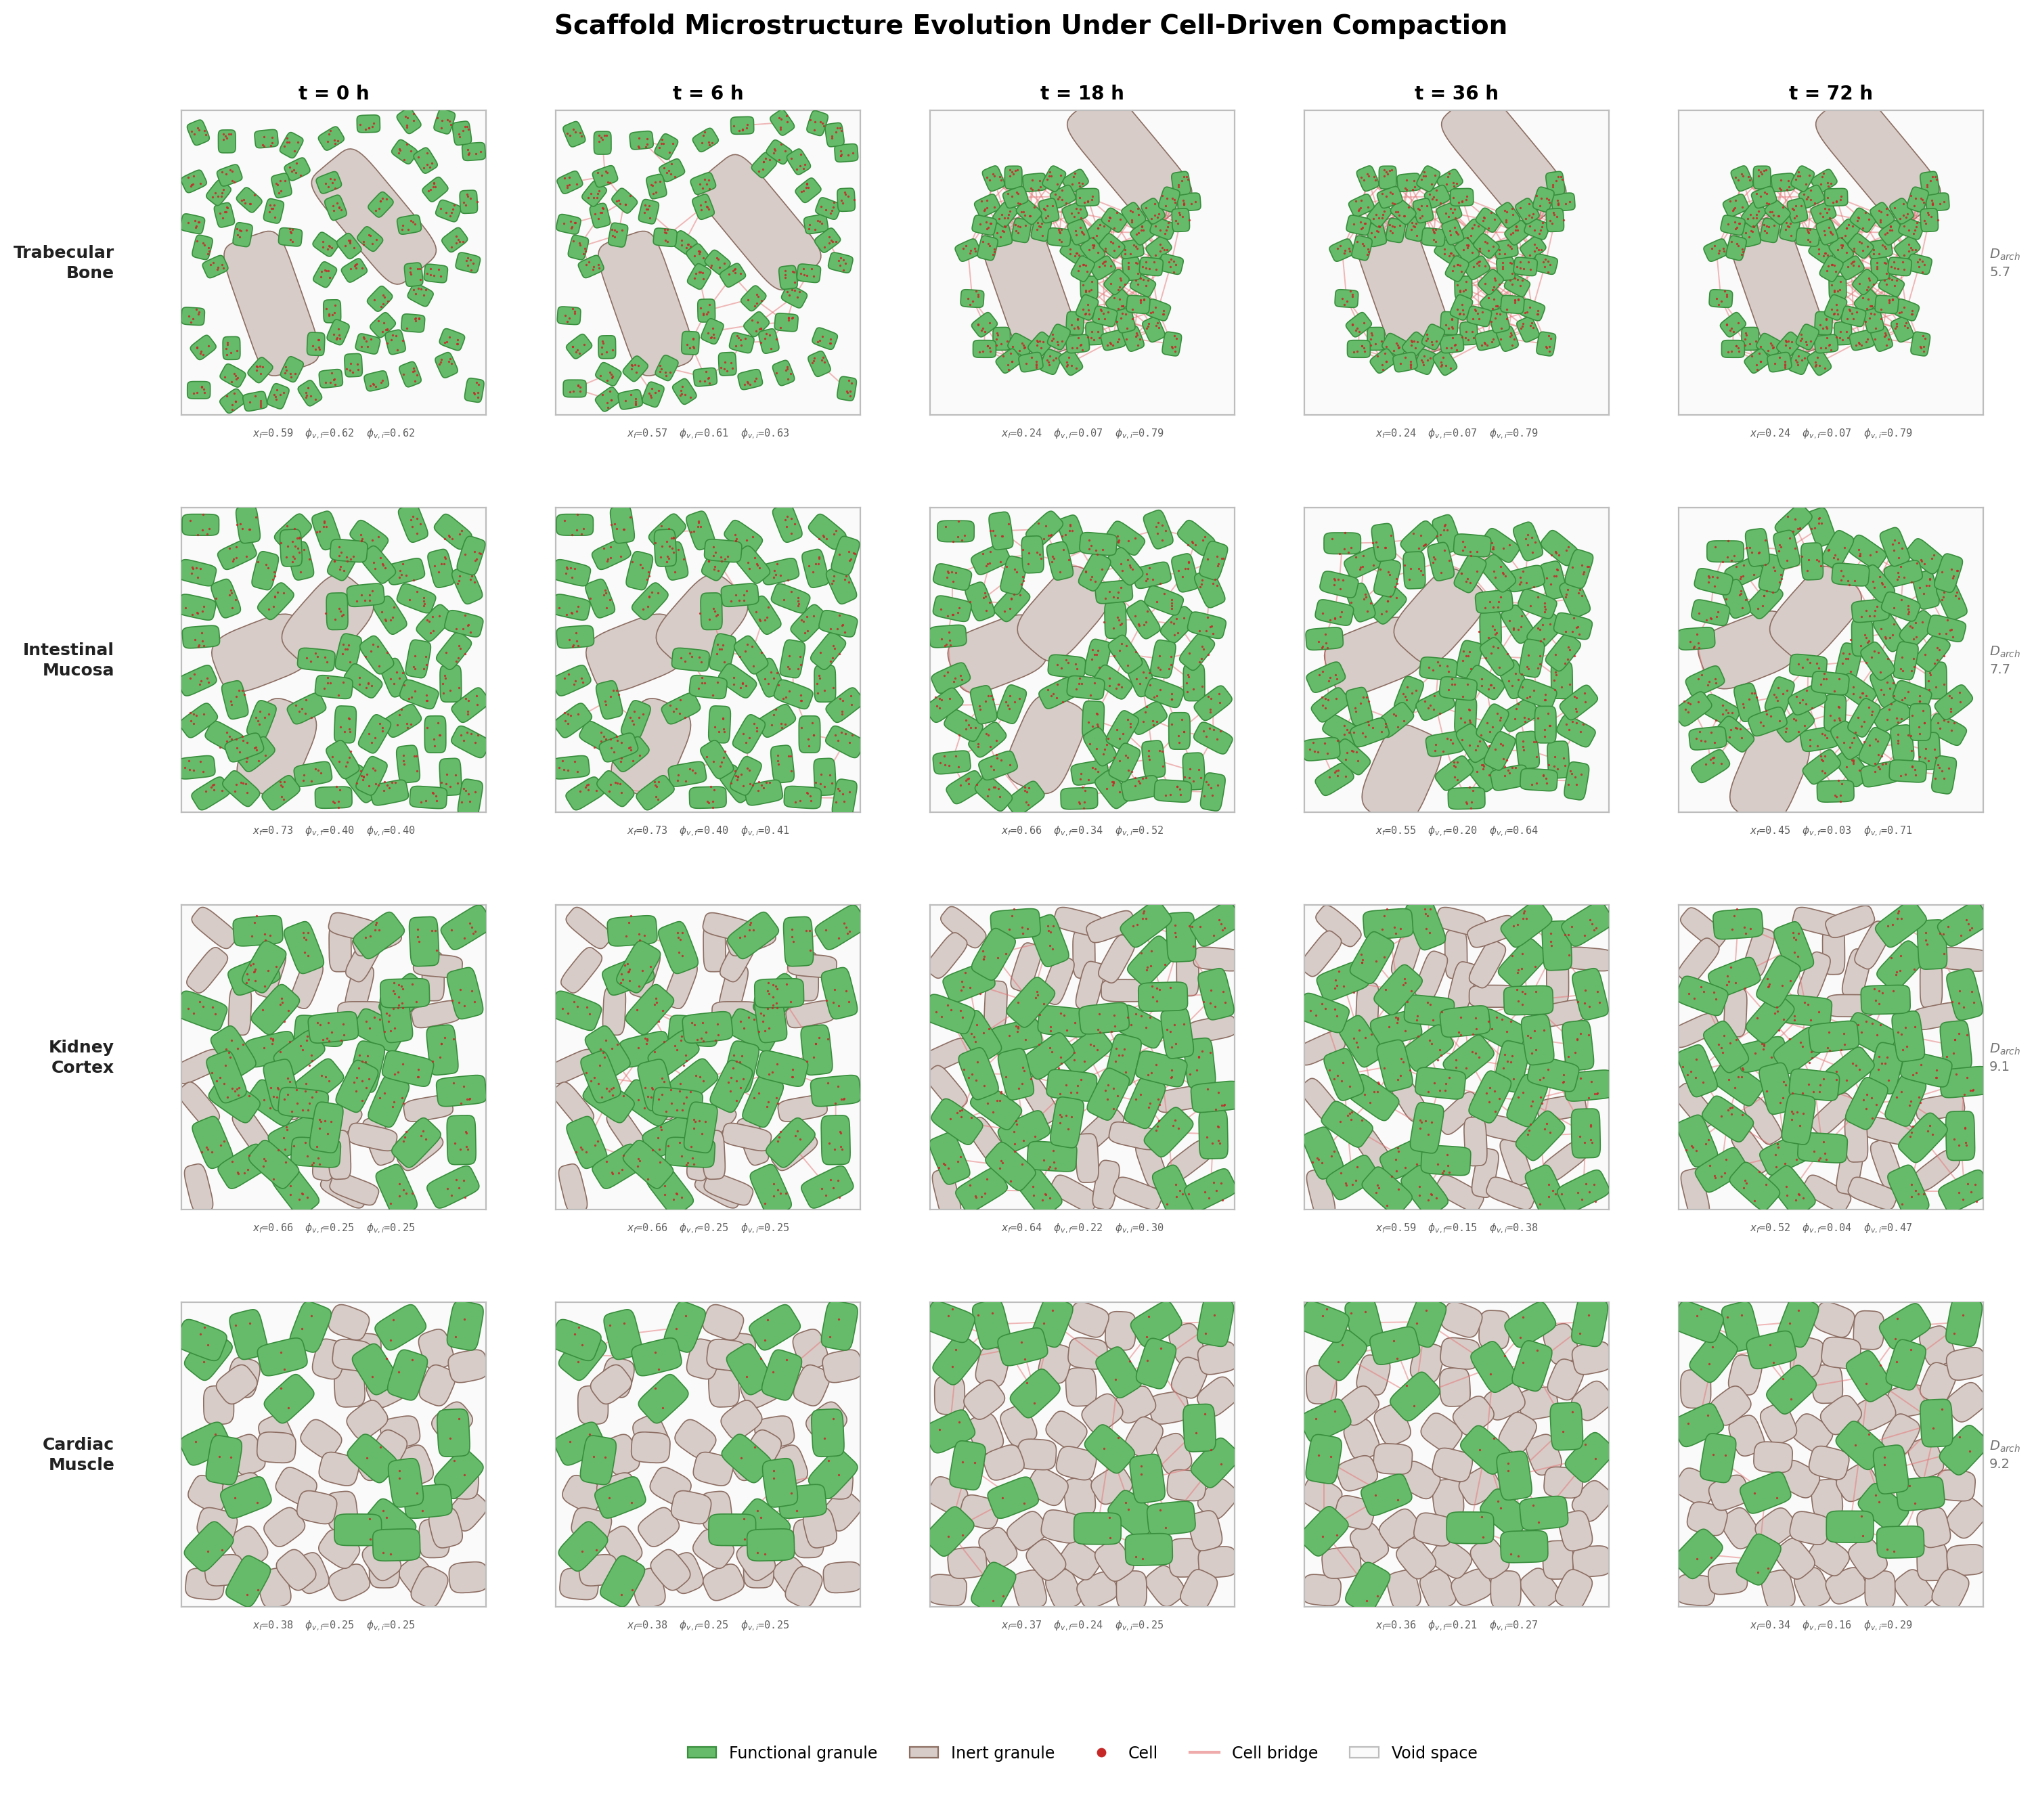
\includegraphics[width=0.95\textwidth]{fig1_scaffold_evolution.png}
  \caption{\textbf{Scaffold microstructure evolution under cell-driven compaction.}
  Timelapse sequences at $t = 0$, $6$, $18$, $36$, and $72$\,h for four organ targets:
  trabecular bone (row~1), intestinal mucosa (row~2), kidney cortex (row~3), and cardiac
  muscle (row~4). Functional (cell-laden) granules shown in green; inert in gray.
  Superellipsoidal shapes with varying aspect ratio and blockiness are visible. The
  functional phase selectively compacts via intercellular bridges while the inert phase
  remains stationary. Compaction increases from cardiac muscle (minimal) to trabecular
  bone (extensive). Inset bar charts show evolving volume fractions ($\phif$, $\phii$,
  $\phiv$), confirming solid conservation and void redistribution.}
  \label{fig:evolution}
\end{figure*}

\begin{figure*}[t]
  \centering
  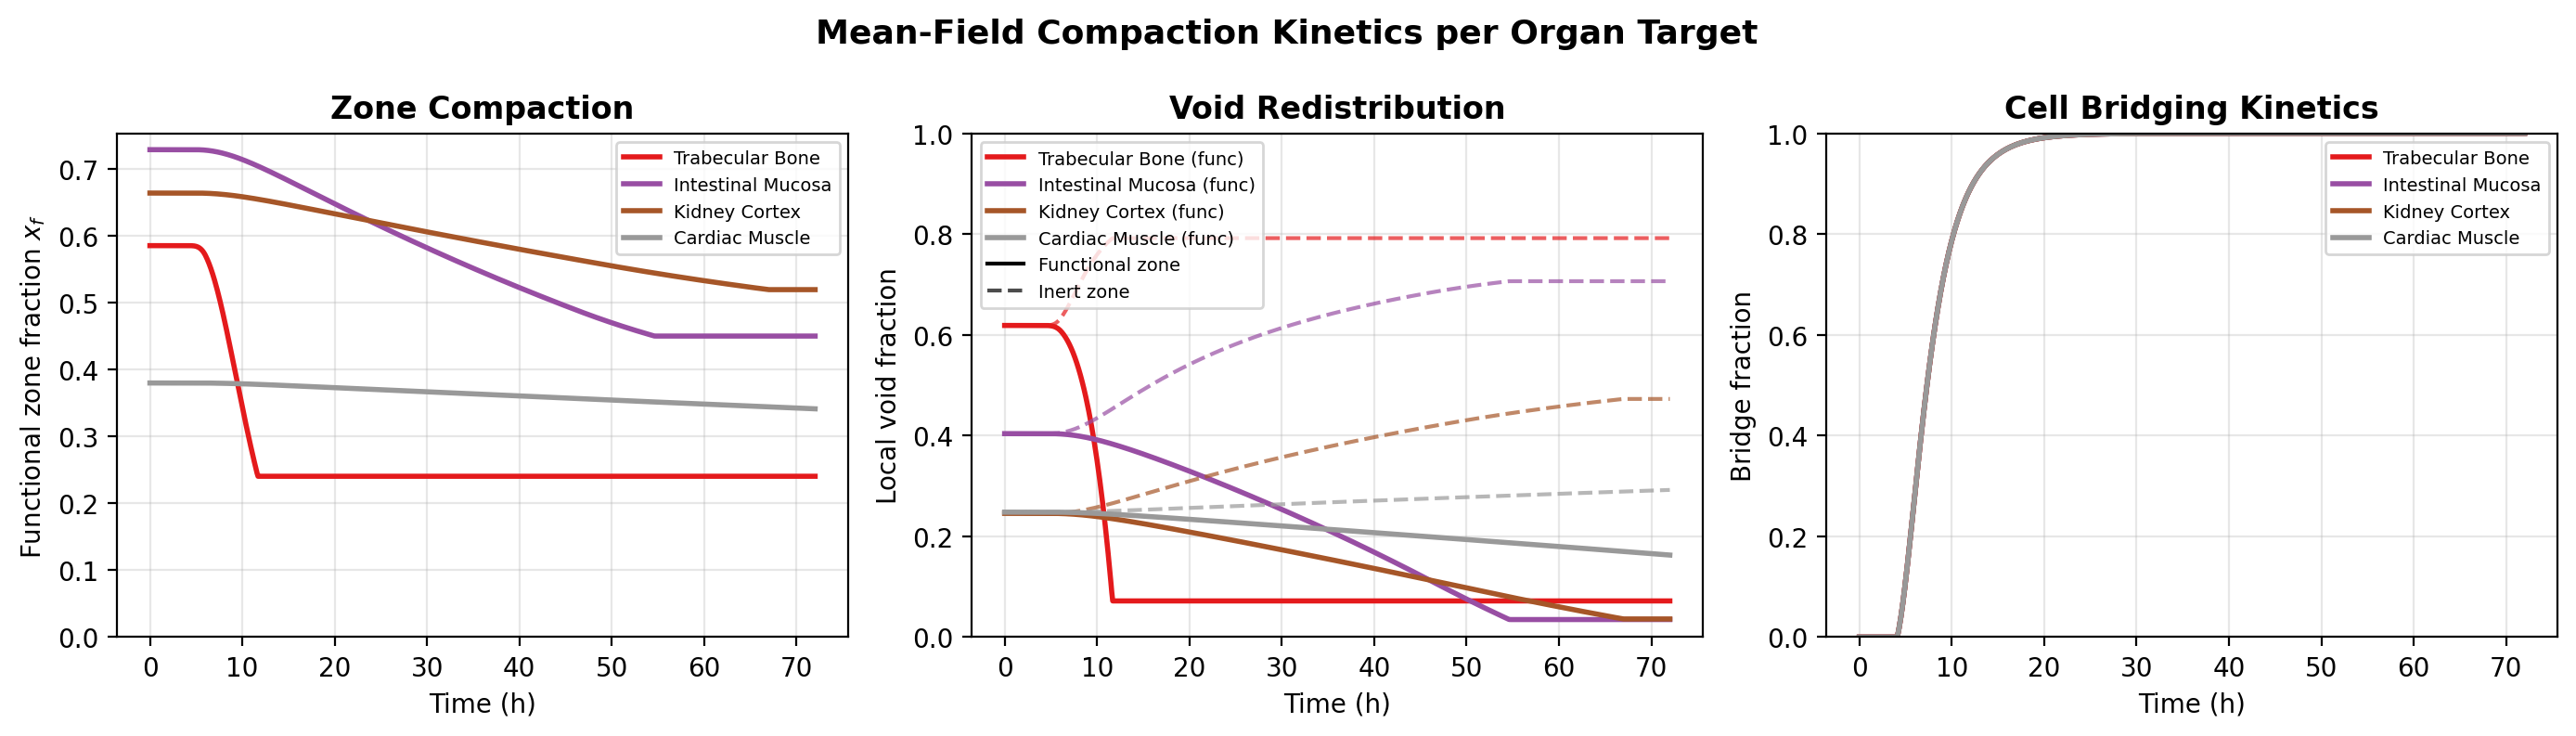
\includegraphics[width=0.92\textwidth]{fig2_kinetics.png}
  \caption{\textbf{Mean-field compaction kinetics per organ target.}
  \textbf{Left:} Functional zone fraction $\xf(t)$. Trabecular bone (red)
  compacts from $\xf = 0.65$ to $0.28$; cardiac muscle (gray) shows minimal
  change. \textbf{Center:} Local void fractions in functional (solid) and
  inert (dashed) zones. Compaction drives functional void fraction toward
  zero while inert zone dilates. \textbf{Right:} Bridge fraction
  $f_\mathrm{bridge}(t)$ with sigmoidal onset at ${\sim}6$\,h (post-attachment)
  and saturation by ${\sim}18$\,h.}
  \label{fig:kinetics}
\end{figure*}

\begin{figure*}[t]
  \centering
  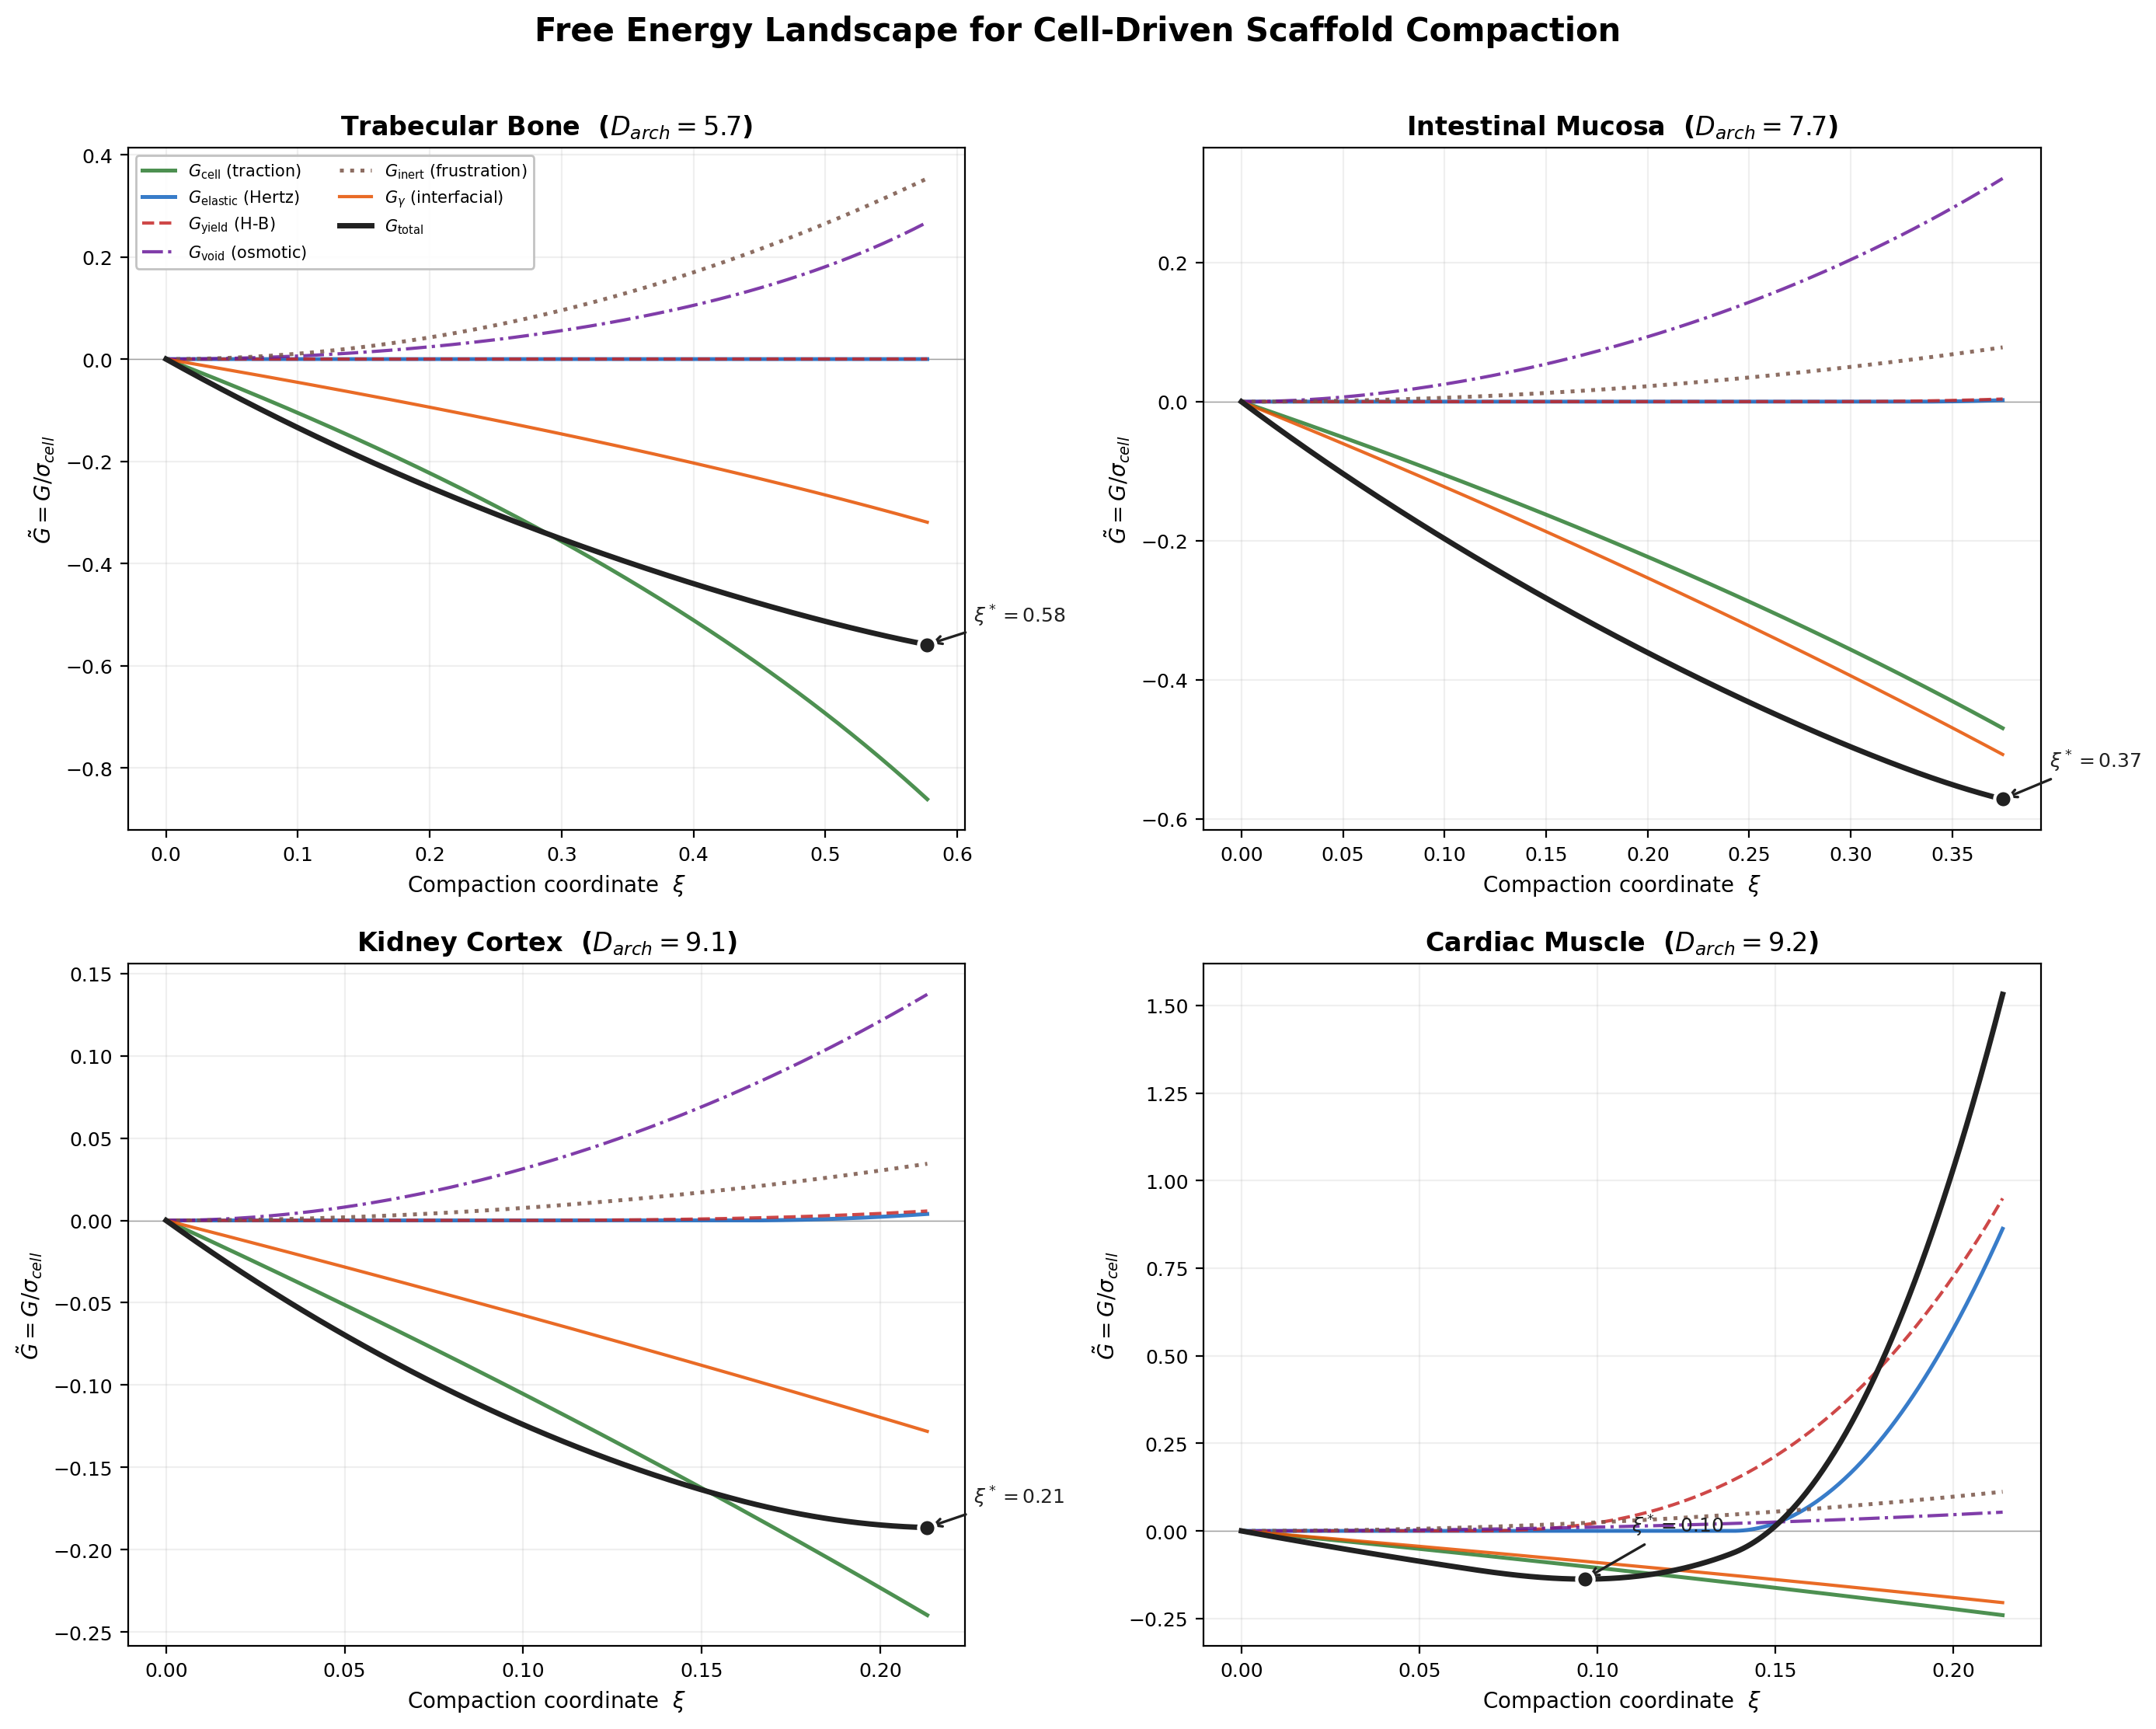
\includegraphics[width=\textwidth]{fig3_energy_landscape.png}
  \caption{\textbf{Free energy landscape for cell-driven scaffold compaction.}
  Normalized $\Gtilde(\xi) = G(\xi)/\sigmacell$ for four organ targets.
  Six contributions: $G_\mathrm{cell}$ (green, driving), $G_\mathrm{elastic}$
  (blue), $G_\mathrm{yield}$ (red dashed), $G_\mathrm{void}$ (purple),
  $G_\mathrm{inert}$ (brown), $G_\gamma$ (orange). Total landscape (black)
  has a single minimum at $\xistar$ (filled circle). Trabecular bone:
  $\xistar = 0.58$, deep minimum (cell traction dominates). Cardiac muscle:
  $\xistar \approx 0.10$, shallow minimum (strong elastic resistance).
  $D_\mathrm{arch}$ denotes architectural distance to target.}
  \label{fig:landscape}
\end{figure*}

\begin{figure}[t]
  \centering
  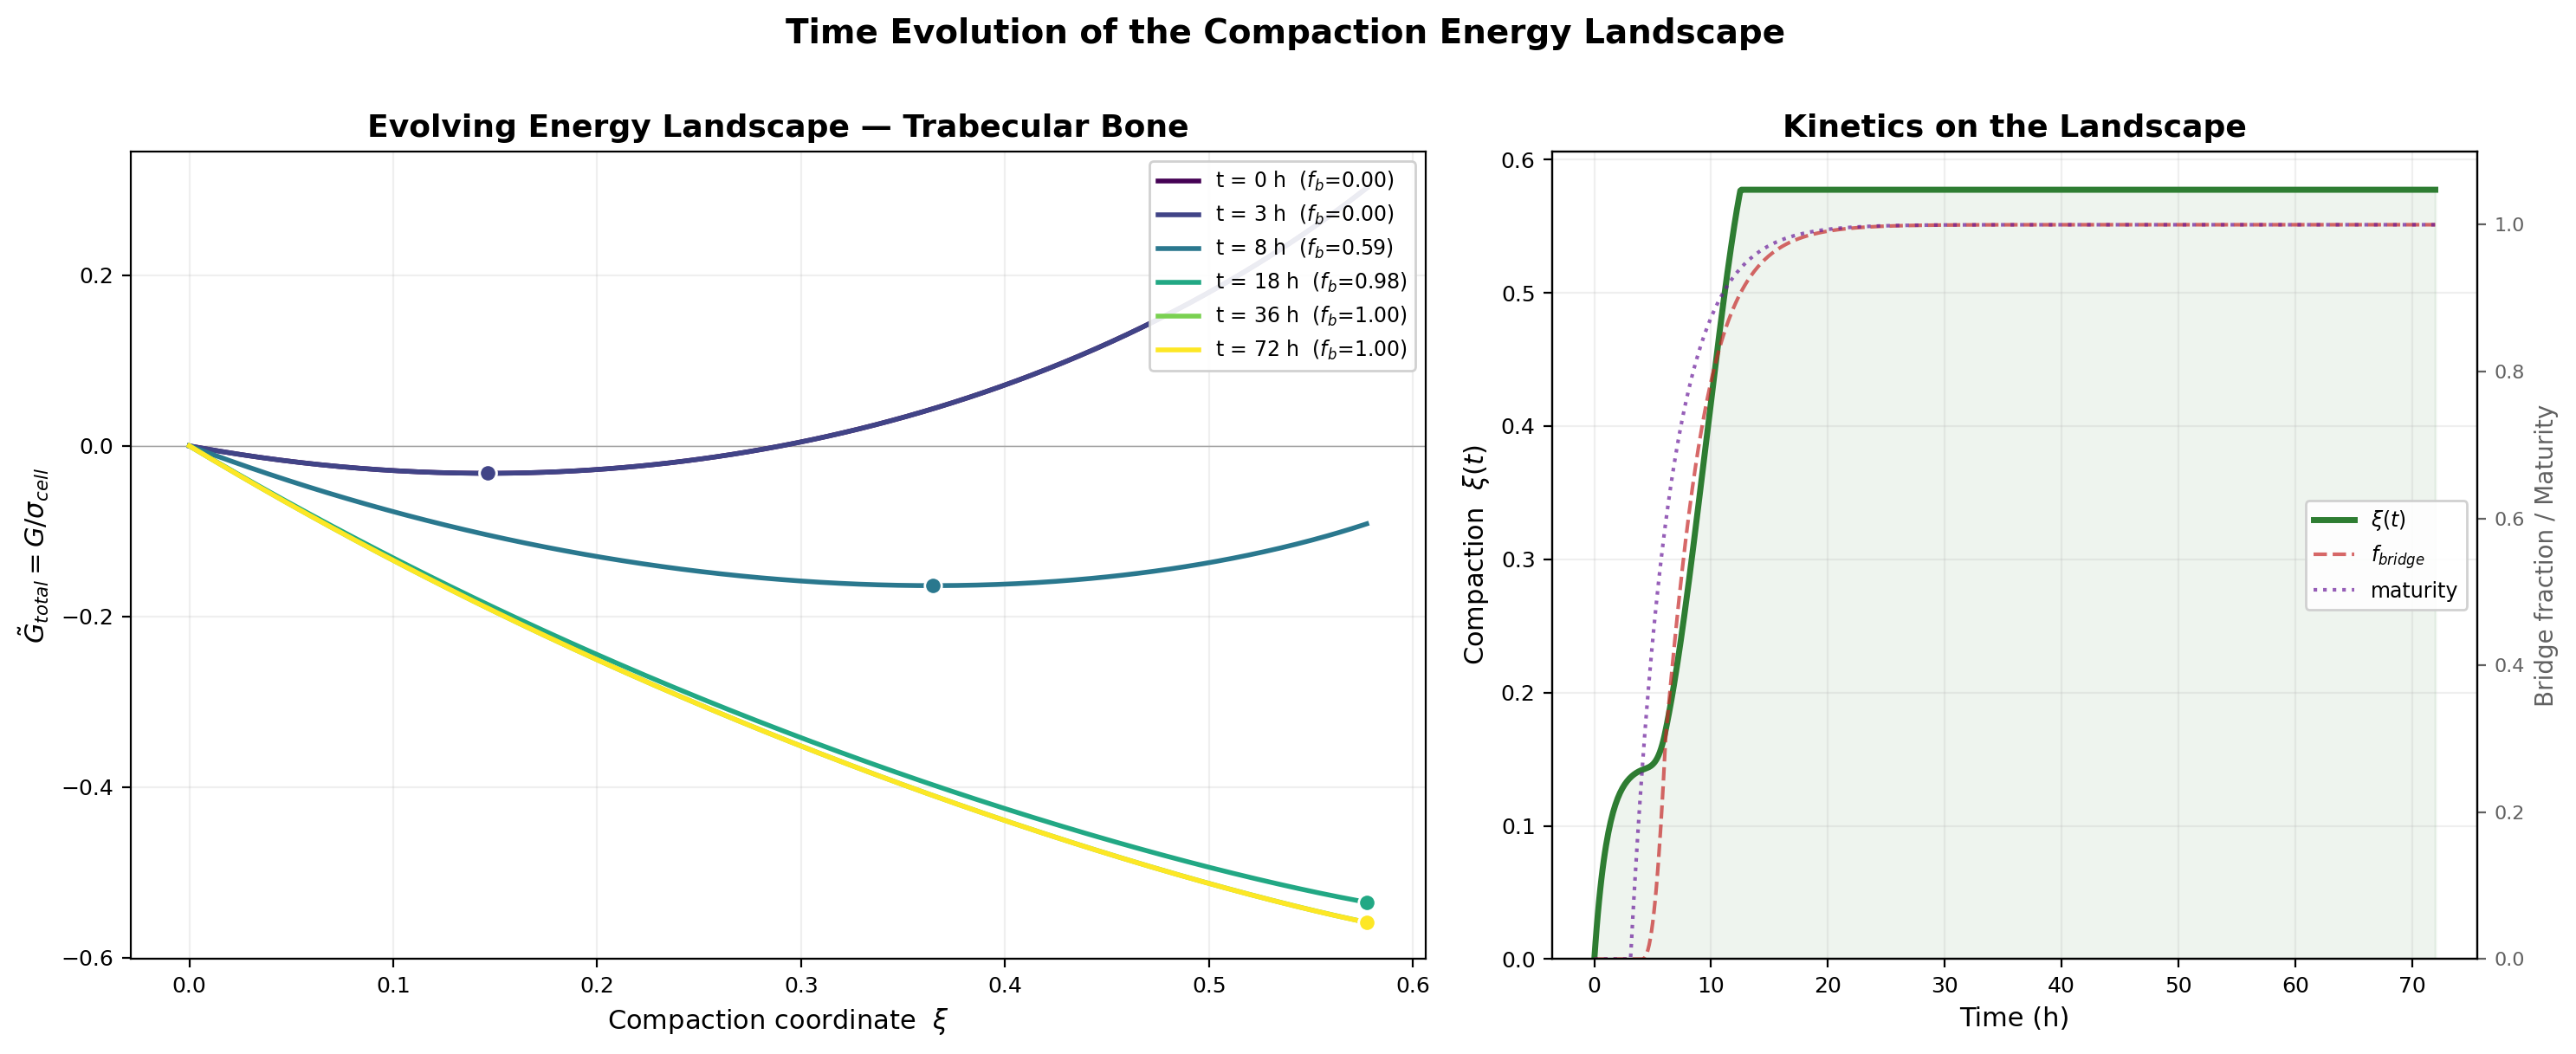
\includegraphics[width=0.92\columnwidth]{fig4_landscape_evolution.png}
  \caption{\textbf{Time evolution of the compaction energy landscape.}
  \textbf{Left:} $\Gtilde(\xi)$ for trabecular bone at six timepoints.
  Bridge formation ($f_b$) progressively deepens the cell traction well;
  filled circles mark instantaneous $\xi(t)$ tracking the evolving minimum.
  \textbf{Right:} $\xi(t)$ (black), $f_\mathrm{bridge}(t)$ (red dashed),
  and FA maturity (gray dotted). Compaction onset lags bridge formation by
  ${\sim}2$\,h due to viscous damping.}
  \label{fig:evolution_landscape}
\end{figure}

\begin{figure*}[t]
  \centering
  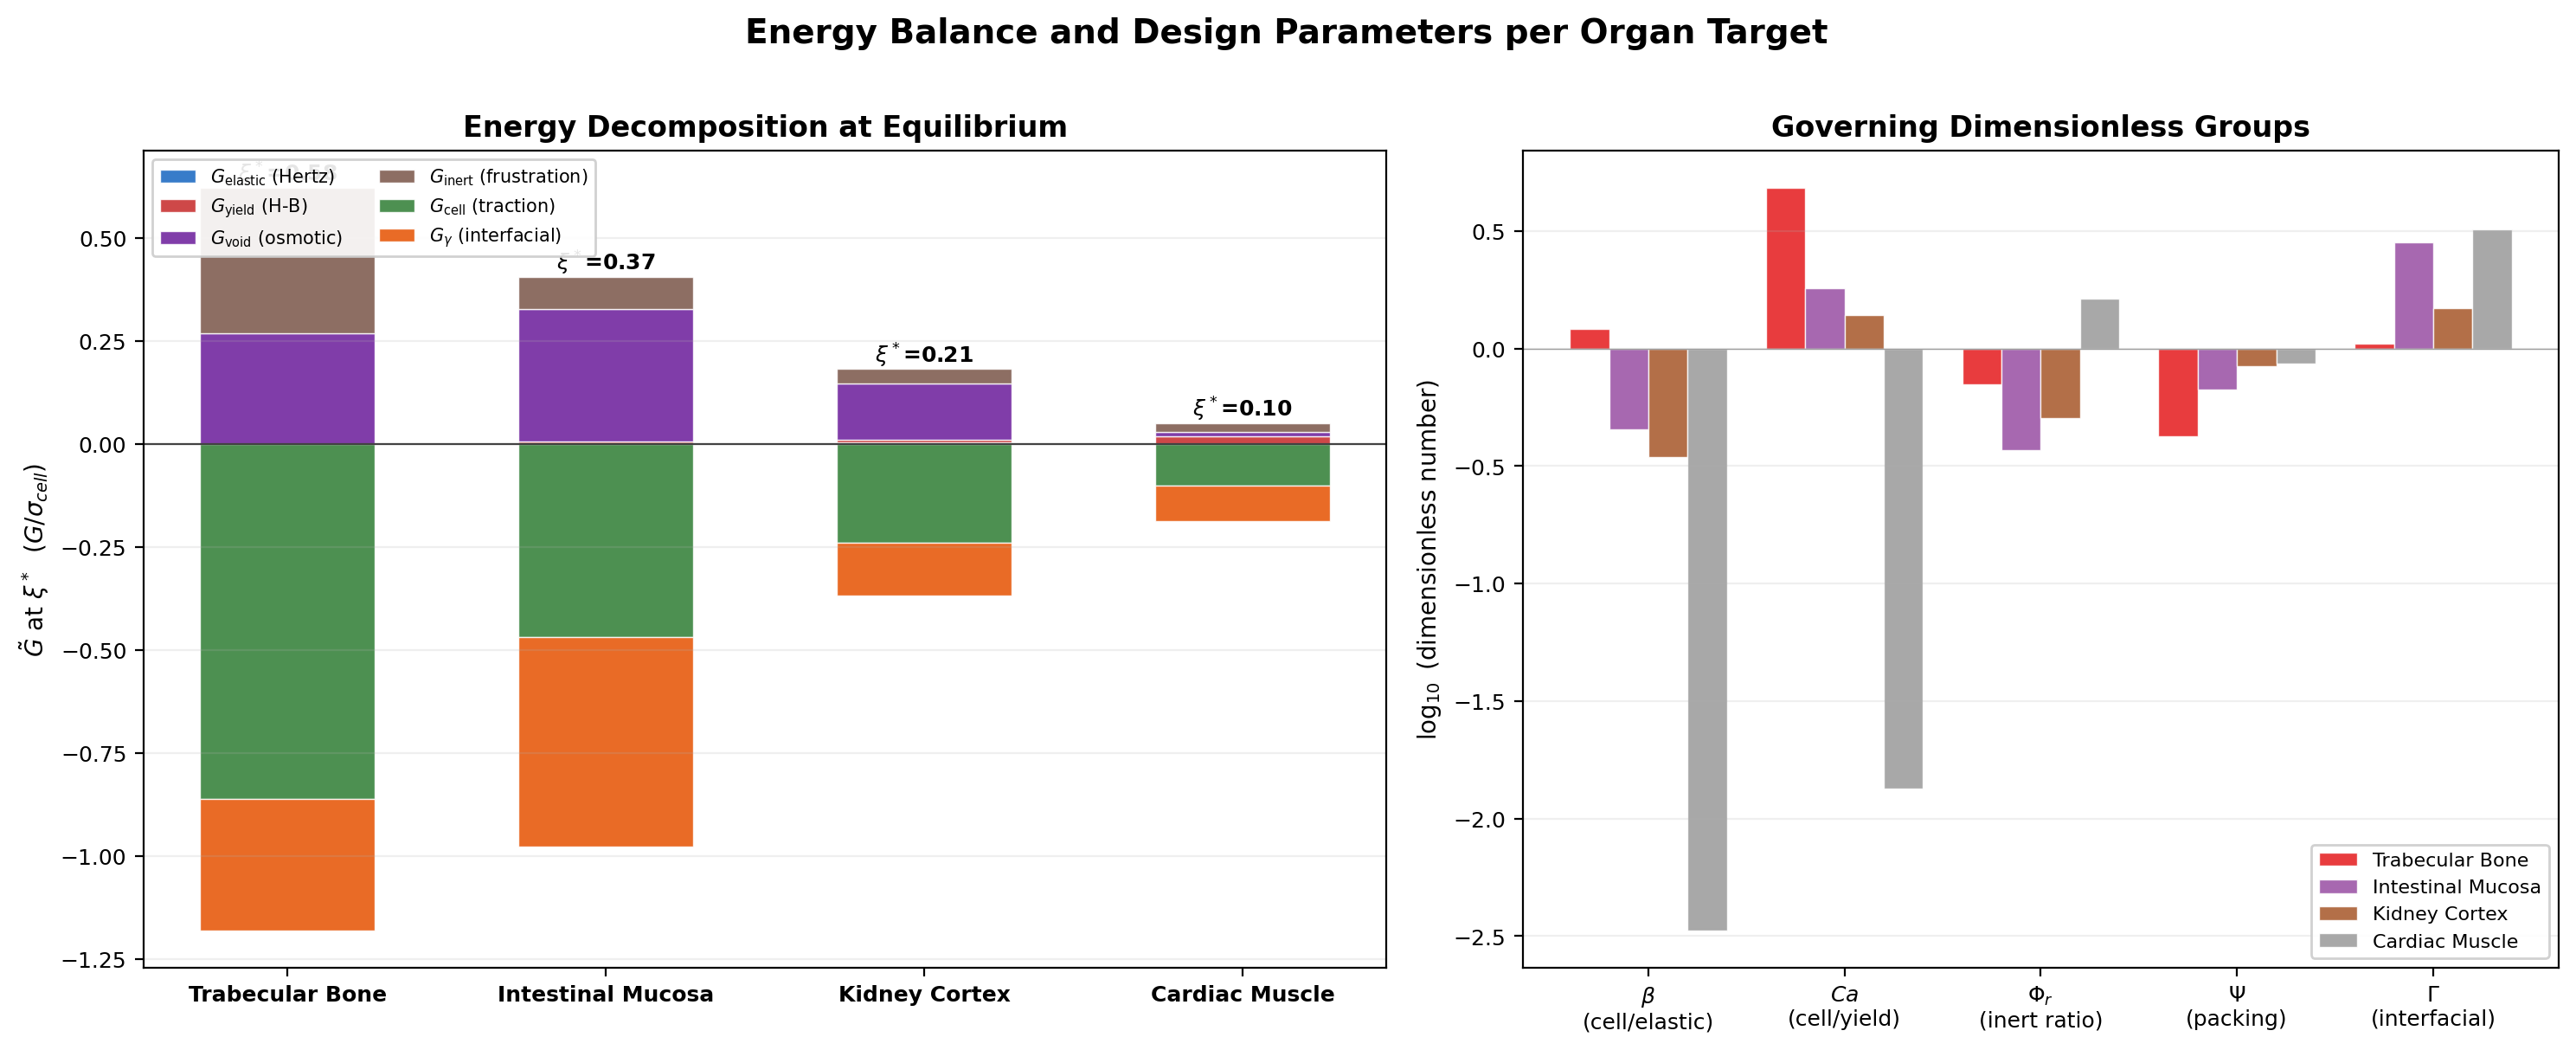
\includegraphics[width=0.92\textwidth]{fig5_energy_decomposition.png}
  \caption{\textbf{Energy decomposition and governing dimensionless groups.}
  \textbf{Left:} Stacked energy at $\xistar$ for four organ targets.
  Negative: driving (green: $G_\mathrm{cell}$; orange: $G_\gamma$).
  Positive: resistance (blue: elastic; red: yield; purple: void; brown:
  frustration). \textbf{Right:} Five dimensionless groups on $\log_{10}$
  scale. Large $\beta$ and Ca correlate with deep compaction; large $\Phi_r$,
  $\Psi$, $\Gamma$ resist it.}
  \label{fig:decomposition}
\end{figure*}

\begin{figure*}[t]
  \centering
  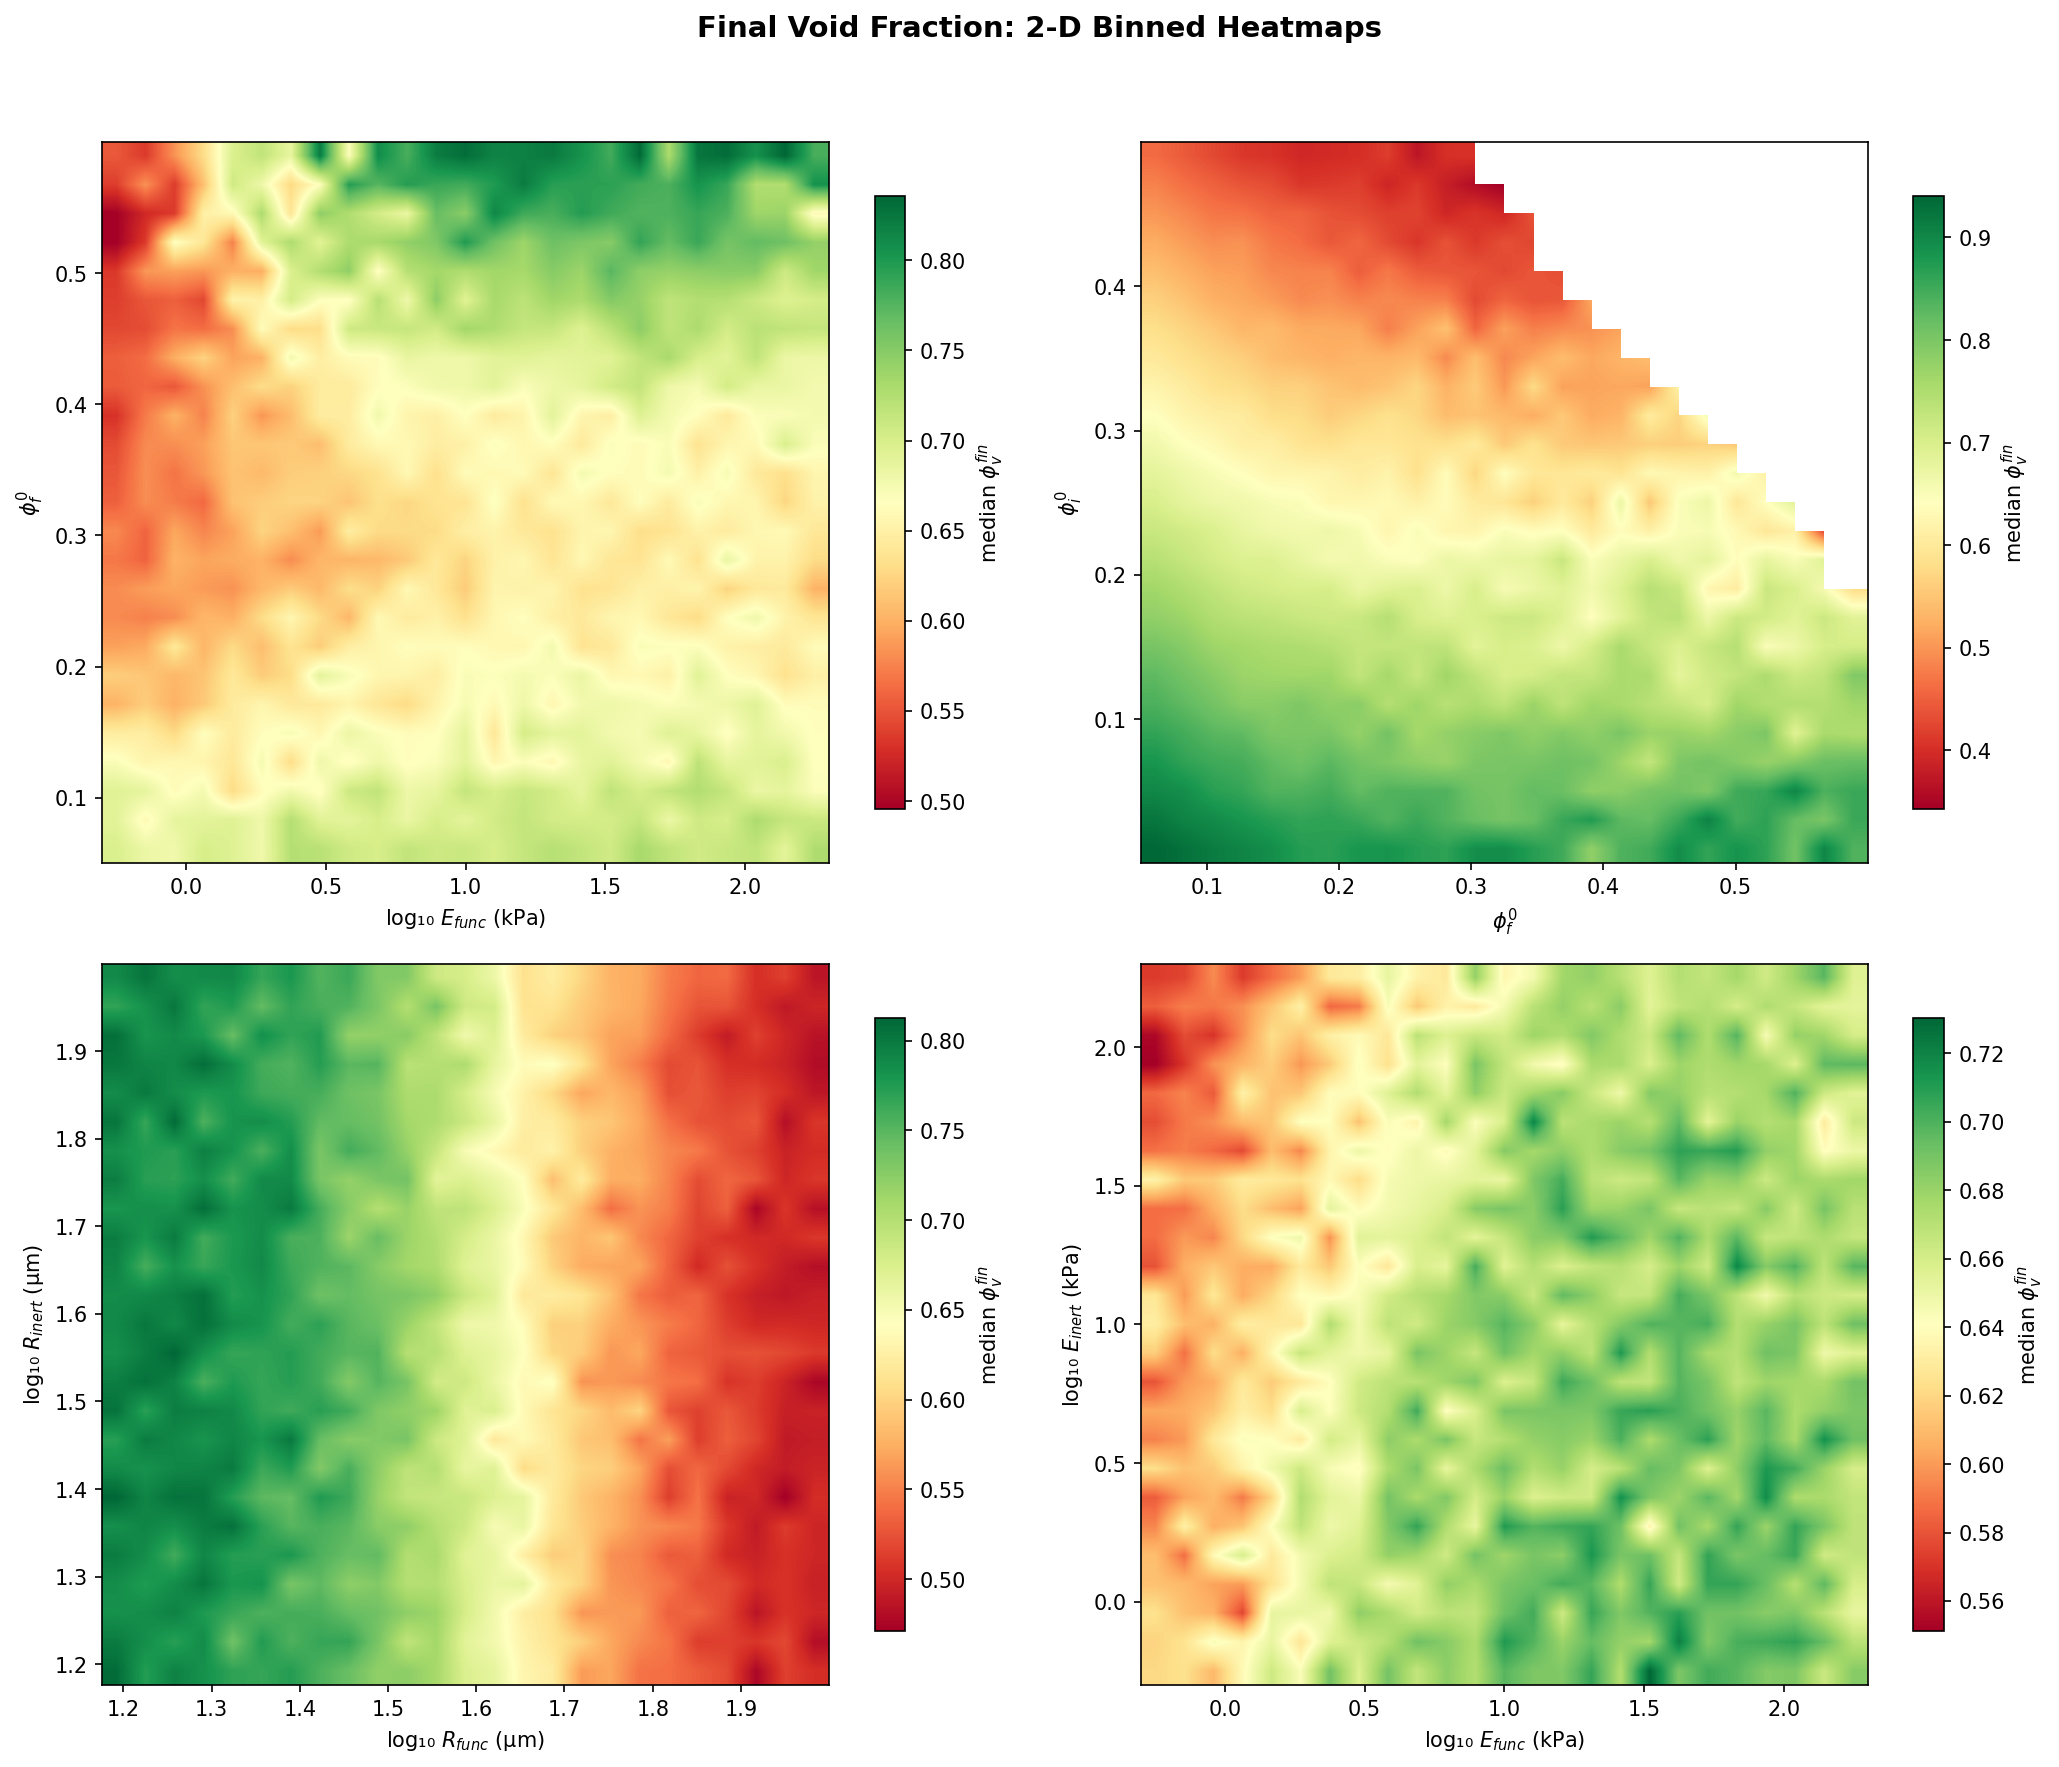
\includegraphics[width=\textwidth]{fig6_design_heatmaps.png}
  \caption{\textbf{Design space for scaffold void fraction.}
  Median $\phiv^{*}$ from 5000-sample Latin hypercube sweep.
  \textbf{Upper left:} Stiffness vs.\ $\phif$; soft granules yield high
  porosity. \textbf{Upper right:} $\phif$ vs.\ $\phii$; diagonal boundary
  from $\phif + \phii \leq 1$. \textbf{Lower left:} Granule radii control
  pore size and permeability. \textbf{Lower right:} Modulus mismatch
  modifies compaction via interfacial stress.}
  \label{fig:heatmaps}
\end{figure*}

% ============================================================
% References
% ============================================================
\bibliographystyle{unsrtnat}
\bibliography{references}

\end{document}
